\documentclass[a4paper,12pt,spanish,oneside]{book}
\special{papersize=210mm,297mm} 
\usepackage{amsmath}
\usepackage{amssymb} 
\usepackage{makeidx}
\usepackage{graphicx}
\usepackage[spanish]{babel}
\usepackage{lipsum}
\makeatletter
\renewcommand\lips@dolipsum{%
  \ifnum\value{lips@count}<\lips@max\relax
    \addtocounter{lips@count}{1}%
    \csname lipsum@\romannumeral\c@lips@count\endcsname
    \lips@dolipsum
  \fi
}
\makeatother

\selectlanguage{spanish}
\usepackage[latin1]{inputenc}

\usepackage{helvet}
\renewcommand{\familydefault}{\sfdefault}

\usepackage{listings}
\usepackage{courier}
\usepackage{xcolor}
\usepackage{framed}

\usepackage{hyperref}
\hypersetup{%
    pdfborder = {0 0 0}
}

\usepackage{supertabular}

\definecolor{lightblue}{RGB}{213,241,250}
\definecolor{javastrings}{rgb}{0.6,0,0} % for strings
\definecolor{javacomments}{rgb}{0.25,0.5,0.35} % comments
\definecolor{javakeywords}{rgb}{0.5,0,0.35} % keywords
\definecolor{javadoc}{rgb}{0.25,0.35,0.75} % javadoc
\lstset{
		 language=Java,
         basicstyle=\footnotesize\ttfamily, % Standardschrift
         numbers=left,               % Ort der Zeilennummern
         numberstyle=\tiny,          % Stil der Zeilennummern
         %stepnumber=2,               % Abstand zwischen den Zeilennummern
         numbersep=5pt,              % Abstand der Nummern zum Text
         tabsize=2,                  % Groesse von Tabs
         extendedchars=true,         %
         breaklines=true,            % Zeilen werden Umgebrochen
         keywordstyle=\color{javakeywords}\bfseries,
		 stringstyle=\color{javastrings},
		 commentstyle=\color{javacomments},
		 morecomment=[s][\color{javadoc}]{/**}{*/},
    	 frame=b,         
 %        keywordstyle=[1]\textbf,    % Stil der Keywords
 %        keywordstyle=[2]\textbf,    %
 %        keywordstyle=[3]\textbf,    %
 %        keywordstyle=[4]\textbf,   \sqrt{\sqrt{}} %
 % 		  stringstyle=\color{white}\ttfamily, % Farbe der String
         showspaces=false,           % Leerzeichen anzeigen ?
         showtabs=false,             % Tabs anzeigen ?
         xleftmargin=17pt,
         framexleftmargin=17pt,
         framexrightmargin=5pt,
         framexbottommargin=4pt,
         backgroundcolor=\color{lightblue},
         showstringspaces=false      % Leerzeichen in Strings anzeigen ?        
 }
 \lstloadlanguages{% Check Dokumentation for further languages ...
         %[Visual]Basic
         %Pascal
         %C
         %C++
         %XML
         %HTML
         Java
 }
 %\DeclareCaptionFont{blue}{\color{blue}} 

%\captionsetup[lstlisting]{singlelinecheck=false, labelfont={blue}, textfont={blue}}
\usepackage{caption}
\DeclareCaptionFont{white}{\color{white}}
\DeclareCaptionFormat{listing}{\colorbox[cmyk]{0.43, 0.35, 0.35,0.01}{\parbox{\textwidth}{\hspace{15pt}#1#2#3}}}
\captionsetup[lstlisting]{format=listing,labelfont=white,textfont=white, singlelinecheck=false, margin=0pt, font={bf,footnotesize}}
\renewcommand{\lstlistlistingname}{�ndice de listados}

\renewcommand{\rmdefault}{ptm}
\textwidth 6.25in
\textheight 9.75in
%\parskip 0.25cm
\parindent 0.0in
\marginparwidth = 0pt
\topmargin -0.3in
\setlength{\oddsidemargin}{0in} 
\setlength{\evensidemargin}{0in}

\begin{document}
 
\begin{titlepage}
\begin{center}
\vspace{5in}
\hrule
\bigskip
\bigskip
{ \huge \bfseries Desarrollo de aplicaciones web con tecnolog�as JSF y JPA}\\[0.4cm]
\bigskip
\hrule
\vspace{3in}
\emph{Autor:} �ngel de Jes�s Vizca�no
\vfill
\end{center}
\end{titlepage}
  

\frontmatter

\mainmatter
\tableofcontents
\chapter{Presentaci\'{o}n}
\label{presentacion}

%{
%\parindent 0em
%\hangafter -6
%\hangindent 1in
%\lipsum
%}

En los �ltimos tiempos se han realizado avances significativos en la simplificaci�n de los desarrollos Java de aplicaciones empresariales. 
La Junta de Castilla y Le�n sigue anclada en tecnolog�as de desarrollo muy desfasadas con respecto a las actuales tecnolog�as. 
Este curso pretende ayudar a los desarrolladores de aplicaciones en el uso de nuevas tecnolog�as que simplifican mucho los desarrollos software. 

Las aplicaciones que desarrollamos habitualmente se componen de tres grandes bloques diferenciados: La capa de vista, la l�gica de negocio y la capa acceso a datos. 
Este curso se orienta a la capa de vista y a la de acceso a datos. JSF da soluci�n a la capa de vista mientras que JPA lo hace en la capa de acceso a datos. 

El enfoque de este curso es eminentemente pr�ctico. El curso se divide en dos grandes bloques, uno referido a JPA y el otro a JSF. 

En el primer bloque aprenderemos como modelar entidades persistentes en base de datos, como crearlax, como acceder a ellas, como modificarlas y como eliminarlas. 

En el segundo aprenderemos a crear interfaces de usuario basadas en el est�ndar JSF, a utilizar platillas reutilizables, a utilizar controles mejorados y a darles soporte Ajax.


\section*{Requisitos del curso} 

Este curso est� dirigido a desarrolladores de aplicaciones J2EE y tiene un enfoque pr�ctico. Por ello se asume que los alumnos tienen conocimientos de programaci�n Java y JSP. 

También se presupone que los alumnos tienen conocimientos de modelado de datos relacionales y lenguaje SQL.

El cambio tecnol�gico nos impone el uso de la versi�n 5 de Java. El uso de esta versi�n no supone apenas cambios en el desarrollo aunque utilizaremos la capacidad 
de anotaciones de esta versi�n en la parte de JPA. Al final del libro hay un apéndice con un resumen de las caracter�sticas de Java 5 que vamos a utilizar y 
ejemplos de cada una de ellas.

Es impensable en la actualidad el trabajar sin la ayuda de algún IDE de desarrollo que nos facilite la labor. Hist�ricamente en la Junta de Castilla y 
Le�n se ha utilizado JDeveloper en cualquiera de sus versiones. En este curso no utilizaremos dicho IDE sino que utilizaremos Eclipse. Este IDE adem�s de 
soportar plenamente las tecnolog�as que vamos a ver en este curso, siendo adem�s mucho m�s vers�til.


  
\chapter{Introducci\'{o}n a las tecnolog\'{i}as JSF 2 y JPA}

 
\chapter{Teor�a de persistencia: JPA}

\section{Breve historia de la persistencia en Java} 

Desde los comienzos de la programaci�n en Java han aparecido tecnolog�as que permitan el acceso y manipulaci�n (persistencia) de datos ubicados en bases de datos relacionales. 
Un breve repaso de las tecnolog�as de persistencia ser�a el siguiente:
 
\subsection*{JDBC}
La especificaci�n JDBC (Java Database Conectivity) permiti� la estandarizaci�n del acceso a las bases de datos. Siempre que hubiese un driver compatible JDBC para una base de datos,
la especificaci�n nos permite el acceso a la misma desde aplicaciones Java. El problema es que aunque JDBC es un est�ndar, SQL no lo es. 
El c�digo SQL cambia para bases de datos distintas (p.e. MySQL y Oracle tienen sintaxis JAVA ligeramente distintas).
\subsection*{EJBs}
Se introdujo en la primera versi�n de J2EE (Java 2 Enterprise Edition) como nueva soluci�n al problema de la persistencia en forma de Entity Bean. 
Delegaban la persistencia al contenedor aunque con carencias en cuanto a portabilidad (configuraci�n XML ad hoc en los despliegues para proveedores espec�ficos), 
coste de red elevado por el acceso RMI a los beans, mapeo insuficiente de las relaciones entre Entity Beans (foreign keys), etc,\ldots
\subsection*{JDO}
Se trat� de un esfuerzo independiente por dar soluci�n al problema de la persistencia. 
Inicialmente requer�a bases de datos orientadas a objetos aunque posteriormente se ampli� a las bases de datos relacionales. 
Requiere de un proceso de \emph{enhancement} del byte code generado por el compilador java que a�ade datos para la gesti�n de la persistencia  en un proceso posterior a la compilaci�n. 
Tambi�n define un lenguaje de consulta orientado a objetos. JDO alcanz� el status de extensi�n JDK aunque nunca el status de est�ndar Java.
\subsection*{JPA}
JPA es el est�ndar de persistencia desarrollado para la plataforma J2EE mediante el est�ndar EJB3. A diferencia de JDO, JPA es un est�ndar Java (JPA 1.0 JSR220 y JPA 2.0 JSR317) 
existiendo una serie de implantaciones tanto comerciales como libres de dicho est�ndar.
JPA permite mapear los objetos y relaciones entre los mismos a tablas relacionales, permitiendo utilizar POJOs (Plain Old Java Objects) 
para mantener las ventajas de la orientaci�n a objetos en el acceso a la base de datos.
\subsection*{JPA2}

\section{Definiciones}
\subsection*{ManagedEntity}
Entidad gestionada por un EntityManager. 
Se trata de todas las clases que se han declarado como entidades.
\subsection*{EntityManagerFactory}
Objeto que se utiliza para interactuar con la base de datos definida en una unidad 
de persistencia. Normalmente se puede identificar con un DataSource. 
Es la encargada de crear los EntityManagers.
\subsection*{EntityManager}
Gestor de entidades persistentes. Recupera, actualiza y mantiene sincronizados 
los ManagedEntities con la base de datos. 
\subsection*{PersistenceUnit} 
Elemento de agrupaci�n l�gica de entidades persistentes que deben de ser tratadas 
de forma igual. Incluye:
\begin{itemize}
\item
Un EntityManagerFactory y todos sus EntityManagers junto con su informaci�n de configuraci�n.
\item
El conjunto de clases gestionadas incluidas en la unidad de persistencia gestionadas por los EntityManagers del EntityManagerFactory.
\item
Metadatos de mapeo que especifica como se mapean las clases en la base de datos.
\end{itemize}

\section{Configuraci�n de la persistencia}
La configuraci�n de la persistencia se realiza mediante el fichero \emph{persistence.xml}.
En el fichero de configuraci�n se especifican el motor de persistencia que se va a utilizar,
 las entidades que se consideran persistentes, as� como diferentes opciones de configuraci�n
 (logs, weaving, \dots).

\section{Modelado de entidades y sus relaciones}

\subsection{XXX}

\section{Consultas}

\section{Consultas avanzadas. Criteria queries.}
 
\chapter[Pr�cticas JPA]{Pr�cticas de modelado JPA}

\section{Enunciado}

Queremos modelar la base de datos de un conjunto de empresas que realizan proyectos para diversos clientes. Cada empresa se 
divide en departamentos que forman una jerarqu�a en �rbol anid�ndose los departmentos. Cada empleado trabaja en un departamento y 
cada departamento tiene un empleado que es responsable del mismo. 

Cada proyecto est� asignado a un departamento o a ninguno si no ha sido asignado a�n. En cada proyecto trabajan los empleados del 
departamento al que est� asignado el proyecto. Cada proyecto tiene asociado un cliente de la cartera global de clientes. 

Un proyecto tiene tres estados:
\begin{itemize}
\item En estudio
\item En desarrollo
\item Entregado
\item Finalizado 
\item Cancelado
\end{itemize} 

El estado inicial del proyecto es \emph{En estudio}. Cuando el proyecto se asocia a un departamento pasa al estado \emph{Desarrollo}.
El proyecto pasa el estado \emph{Entregado} cuando se entrega al cliente. Se debe registrar la fecha de entrega al cliente al alcanzar 
dicho estado. Cuando el cliente acepta el proyecto (despu�s de probarlo) el proyecto pasa al estado \emph{Finalizado}.
El cliente puede rechazar una entrega del proyecto con lo que el proyecto pasa al estado \emph{En desarrollo}.
Una vez que el proyecto est� entregado el cliente puede pedir mejoras para la siguiente versi�n del proyecto. En este caso el proyecto pasa
al estado \emph{En estudio} con un n� de versi�n superior y vuelven a realizar todas las fases.
En cualquier momento del proceso se puede cancelar un proyecto pasando el estado del mismo a \emph{Cancelado} y grab�ndose el motivo y la fecha 
de cancelaci�n.


\begin{figure}[h]
\centering
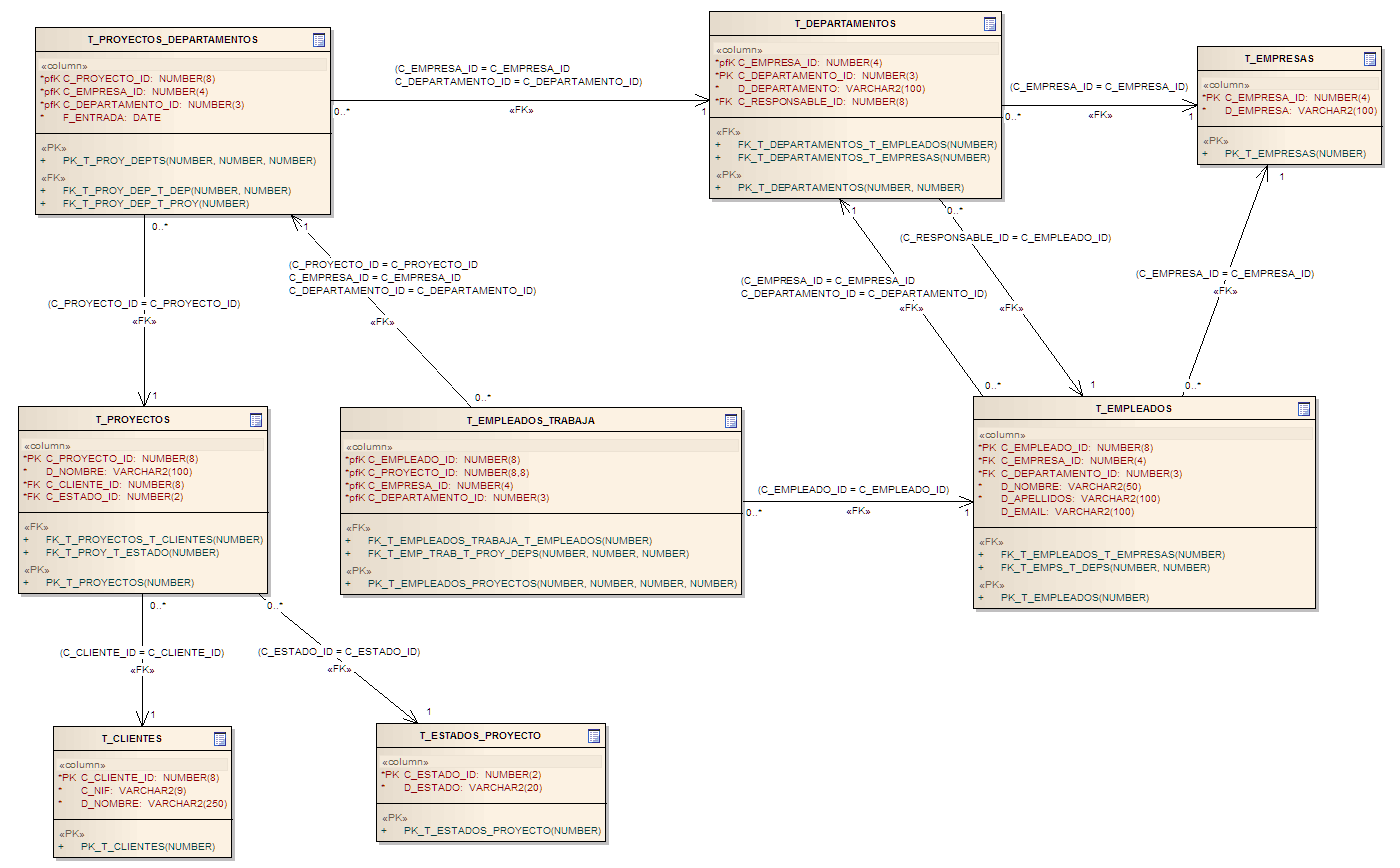
\includegraphics[width=6in]{cap03/PRUE.png}  
\caption{Modelo de datos de la pr�ctica}
\label{cap03:fig01}
\end{figure}
 
\section{Pr�ctica 1}
En esta pr�ctica vamos a modelar cada una de las entidades que aparecen en el enunciado:

\lstinputlisting[label=cliente.java,caption=Cliente.java]{../practicas/practica1/src/practica1/modelo/Cliente.java}
\lstinputlisting[label=departamento.java,caption=Departamento.java]{../practicas/practica1/src/practica1/modelo/Departamento.java}
\lstinputlisting[label=departamentoPK.java,caption=DepartamentoPK.java]{../practicas/practica1/src/practica1/modelo/DepartamentoPK.java}
\lstinputlisting[label=empleado.java,caption=Empleado.java]{../practicas/practica1/src/practica1/modelo/Empleado.java}
\lstinputlisting[label=empresa.java,caption=Empresa.java]{../practicas/practica1/src/practica1/modelo/Empresa.java}
\lstinputlisting[label=estado.java,caption=Estado.java]{../practicas/practica1/src/practica1/modelo/Empresa.java}
\lstinputlisting[label=proyecto.java,caption=Proyecto.java]{../practicas/practica1/src/practica1/modelo/Proyecto.java}
\lstinputlisting[label=proyectoDepartamentoPK.java,caption=ProyectoDepartamentoPK.java]{../practicas/practica1/src/practica1/modelo/ProyectoDepartamentoPK.java}
\lstinputlisting[label=proyectoDepartamento.java,caption=ProyectoDepartamento.java]{../practicas/practica1/src/practica1/modelo/ProyectoDepartamento.java}

\section{Pr�ctica 2}
 
\chapter{Teor�a de vista: JSF 2}

\section{Definiciones}

\section{Configuraci\'{o}n de aplicaciones Web con tecnolog�aa JSF 2}

\section{Beans gestionados}

\section{P�ginas web en JSF 2}

\subsection{Etiquetas de JSF 2}

\subsection{Lenguaje de Expresiones (EL)}

\section{Navegaci�n}

\section{Conversi�n}

\section{Validaci�n}

\section{Gesti�n de errores}

\section{Plantillas en JSF. Facelets}

\section{Utilizaci�n de librer�as JSF de terceros: Primefaces}

 

\chapter[Pr\'{a}ctica 2]{Pr\'{a}ctica de desarrollo de una aplicaci\'{o}n web JSF 2}
 

\chapter[Pr\'{a}ctica 2]{Pr\'{a}ctica de implementaci\'{o}n de una aplicaci\'{o}n web compleja utilizando JPA, JSF 2, Facelets y Primefaces.}


 
  
\chapter{Conceptos avanzados en el modelado de relaciones JPA}

 
  
\chapter{Conceptos avanzados en la intercomunicaci\'{o}n de de beans y navegaci\'{o}n avanzada en JSF}

 
 
\chapter{Utilizaci\'{o}n del framework del Servicio de Inform\'{a}tica de la Consejer\'{i}a de Sanidad en aplicaciones Web}

\section{Configuraci\'{o}n}

\section{Seguridad}

\section{Gesti\'{o}n de componentes de negocio}

 

\chapter[Pr�ctica 4]{Pr�ctica de adaptaci�n de una aplicaci�n compleja al framework del Servicio de Inform�tica de la Consejer�a de Sanidad}

  

\appendix
\clearpage
\chapter[Ap�ndice A]{Instalaci�n del entorno de pr�cticas}

Para el desarrollo de las pr�cticas se va a utilizar eclipse como entorno integrado de desarrollo, 
Eclipselink como gestor de persistencia JPA y Tomcat 6 como contenedor de\emph{Servlets} para el despliegue de  aplicaciones Web.

Todas estas aplicaciones y librer�as se eoncontrar�n en el servidor Web: 

\emph{http://jsnsc52p194.jcyl.red/curso/software/curso.zip}

Lo primero que haremos es descomprimir el fichero curso.zip en le directorio C:\textbackslash:Curso. Esto nos crear� una serie 
de directorios:
\begin{itemize}
  \item docs
  \begin{itemize}
    \item manual.pdf
	\end{itemize}
  \item software
  \begin{itemize}
    \item apache-tomcat-6.0.29
    \item eclipse-jee-juno-SR2-win32
    \item sqldeveloper-3.2.2
  \end{itemize}
  \item libs
  \begin{itemize}
    \item eclipselink-2.4 
    \item db-derby-10.9.1.0
    \item facelets-1.1.15
    \item jstl-1.2
    \item junit-4.10
    \item myfaces-core-2.1.10-bin
    \item primefaces-3.15
  \end{itemize}
  \item practicas
  \begin{itemize}	
    \item bbdd
    \item practica1
    \item practica2
    \item practica3
    \item practica4
    \item practica5
  \end{itemize}
\end{itemize}


\chapter[Ap�ndice B]{Expression Language [EL]}

\section{Introduction}

\textit{JavaServer} \textit{Faces} provides an expression language
(\textit{JSF} EL) that is used in web application pages to access the
JavaBeans components in the page \textit{bean} and in other beans
associated with the web application, such as the session \textit{bean}
and the application \textit{bean}. 

\section{\textit{JavaServer Faces} EL Expression Syntax}

\textit{JSF} EL can be used to bind JavaBeans to component properties to
simplify how the components access data from various sources.
\textit{JSF} EL expressions use the syntax
\emph{\#\{expr\};} 

The syntax of a value binding expression is identical to the syntax of
an expression language expression defined in the \textit{JavaServer}
Pages Specification (version 2.0), sections 2.3 through 2.9, with the
following exceptions:

\begin{itemize}
\item The expression delimiters for a value binding expression are
\emph{\#\{} and \emph{\}}
instead\newline
of \emph{\$\{} and \emph{\}}. 
\item Value binding expressions do not support JSP expression language
functions. 
\end{itemize}
In addition to the differences in delimiters, the two expression types
have the following semantic differences:

\begin{itemize}
\item During \textit{render}ing, value binding expressions are evaluated
by the \textit{JavaServer} \textit{Faces} implementation (via calls to
the \emph{getValue} method) rather than by the
compiled code for a page. 
\item Value binding expressions can be evaluated programmatically, even
when a page is not present. 
\item Value binding expression evaluation leverages the facilities of
the configured \emph{VariableResolver} and
\emph{PropertyResolver} objects available through
the \emph{Application} object for the current web
application, for which applications can provide plug-in replacement
classes that provide additional capabilities. 
\item If a value binding expression is used for the value property of an
\emph{EditableValueHolder} component (any input
field component), the expression is used to modify the referenced value
rather than to retrieve it during the Update Model Values phase of the
\textit{request} processing lifecycle. \newline
\end{itemize}
Examples of valid value binding expressions include: 

\ \ \ \#\{Page1.name\}

\ \ \ \#\{Foo.bar\}

\ \ \ \#\{Foo[bar]\}

\ \ \ \#\{Foo[bar]\}

\ \ \ \#\{Foo[3]\}

\ \ \ \#\{Foo[3].bar\}

\ \ \ \#\{Foo.bar[3]\}

\ \ \ \#\{Customer.status == VIP\}

\ \ \ \#\{(Page1.City.farenheitTemp - 32) * 5 / 9\}

\ \ \ Reporting Period: \#\{Report.fromDate\} to \#\{Report.toDate\}

For value binding expressions where the
\emph{setValue} method is going to be called (for
example, for \emph{text} property bindings for input
fields during Update Model Values), the syntax of a value binding
expression is limited to one of the following forms, where
\emph{expr-a} is a general expression that evaluates
to some object, and \emph{value-b} is an identifier:

\ \ \ \#\{expr-a.value-b\}

\ \ \ \#\{expr-a[value-b]]

\ \ \ \#\{value-b\}

\section{\bfseries Get Value Semantics}

When the \emph{getValue} method of a
\emph{ValueBinding} instance is called (for example,
when an expression on a JSP tag attribute is being evaluated during the
\textit{render}ing of the page), and the expression is evaluated, and
the result of that evaluation is returned, evaluation takes as follows:

\begin{itemize}
\item The expression language unifies the treatment of the
\emph{.} and \emph{[]} operators.
\emph{expr-a.expr-b} is equivalent to
\emph{a[expr-b]}; that
is, the expression \emph{expr-b} is used to
construct a literal whose value is the identifier, and then the
\emph{[]} operator is used with that value. 
\item The left-most identifier in an expression is evaluated by the
\emph{VariableResolver} instance that is acquired
from the Application instance for this web application. If the value on
the left side of the \emph{.} or
\emph{[]} operator is a
\emph{RowSet}, the object on the right side is
treated as a column name. See the next section for a more complete
evaluation description of these operators. 
\item Each occurrence of the \emph{.} or
\emph{[...]} operators in an expression is evaluated
by the \emph{PropertyResolver }instance that is
acquired from the \emph{Application} instance for
this web application. 
\item Properties of variables are accessed by using the
\emph{.} operator and can be nested arbitrarily. 
\end{itemize}

\section{\bfseries Set Value Semantics}

When the \emph{setValue} method of a
\emph{ValueBinding} is called (for example, for
\emph{text} property bindings for input fields
during Update Model Values), the syntax of the value binding
restriction is restricted as described in the previous section. The
implementation must perform the following processing to evaluate an
expression of the form \emph{\#\{expra.value-b\}} or
\emph{\#\{expr-a[value-b]\}}:

\begin{itemize}
\item Evaluate \emph{expr-a} into
\emph{value-a}. 
\item If \emph{value-a} is null, throw
\emph{PropertyNotFoundException}. 
\item If \emph{value-b} is null, throw
\emph{PropertyNotFoundException}. 
\item If \emph{value-a} is a Map, call
\emph{value-a.put(value-b, new-value)}. 
\item If \emph{value-a} is a
\emph{List} or an array: 

\begin{itemize}
\item Coerce \emph{value-b} to
\emph{int}, throwing
\emph{ReferenceSyntaxException} on an error. 
\item Attempt to execute \emph{value-a.set(value-b,
new-value)} or \emph{Array.set(value-b, new-value)}
as appropriate. 
\item If \emph{IndexOutOfBoundsException }or
\emph{ArrayIndexOutOfBoundsException} is thrown,
throw \emph{PropertyNotFoundException}. 
\item If a different exception was thrown, throw
\emph{EvaluationException}. \newline
\end{itemize}
\item Otherwise (\emph{value-a} is a JavaBeans
object): 

\begin{itemize}
\item Coerce \emph{value-b} to
\emph{String}. 
\item If \emph{value-b} is a writeable property of
\emph{value-a} (as per the JavaBeans Specification),
call the setter method (passing \emph{new-value}).
Throw \emph{ReferenceSyntaxException }if an
exception is thrown. 
\item Otherwise, throw
\emph{PropertyNotFoundException}. \newline
\end{itemize}
\end{itemize}
If the entire expression consists of a single identifier, the following
rules apply:

\begin{itemize}
\item If the identifier matches the name of one of the implicit objects
described below,\newline
throw \emph{ReferenceSyntaxException}. 
\item Otherwise, if the identifier matches the key of an attribute in
\textit{request} scope,\newline
session scope, or application scope, the corresponding attribute value
will be\newline
replaced by \emph{new-value}. 
\item Otherwise, a new \textit{request} scope attribute will be created,
whose key is the\newline
identifier and whose value is \emph{new-value}.
\newline
\end{itemize}
\section{\bfseries Implicit Objects }

The expression language defines a set of implicit objects: 

\begin{itemize}
\item \emph{\textit{FacesContext}} - The
\textit{FacesContext} instance for the current \textit{request}. 
\item \emph{param} - Maps a \textit{request}
parameter name to a single value. 
\item \emph{paramValues} - Maps a \textit{request}
parameter name to an array of values. 
\item \emph{header} - Maps a \textit{request} header
name to a single value. 
\item \emph{headerValues} - Maps a \textit{request}
header name to an array of values. 
\item \emph{cookie} - Maps a cookie name to a single
cookie. 
\item \emph{initParam} - Maps a context
initialization parameter name to a single value. \newline
\end{itemize}
Objects that allow access to various scoped variables:

\begin{itemize}
\item
\emph{\textit{request}}\emph{Scope}
- Maps \textit{request}{}-scoped variable names to their values. 
\item \emph{sessionScope} - Maps session-scoped
variable names to their values. 
\item \emph{applicationScope} - Maps
application-scoped variable names to their values. 
\end{itemize}
When an expression references one of these objects by name, the
appropriate object is returned. An implicit object takes precedence
over an attribute that has the same name. For example,
\emph{\#\{}\emph{\textit{FacesContext}}\emph{\}}
returns the \emph{\textit{FacesContext}} object,
even if there is an existing
\emph{\textit{FacesContext}} attribute containing
some other value.

\section{\bfseries Literals }

The expression language defines the following literals: 

\begin{itemize}
\item Boolean: \emph{true} and
\emph{false} 
\item Integer: as in Java 
\item Floating point: as in Java 
\item String: with single and double quotes;
\emph{} is escaped as
\emph{{\textbackslash}},
\emph{ }is escaped as
\emph{{\textbackslash}}, and
\emph{{\textbackslash}} is escaped as
\emph{{\textbackslash}{\textbackslash}}. 
\item Null: \emph{null}
\end{itemize}

\section{\bfseries Operators }

In addition to the \emph{.} and
\emph{[]} operators discussed above in
\href{http://developers.sun.com/docs/jscreator/help/jsp-jsfel/jsf_expression_language_intro.html#getvaluesemantics}{Get
Value Semantics} and the section after that one, the expression
language provides the following operators: 

\begin{itemize}
\item Arithmetic: \emph{+},
\emph{{}- }\textit{(binary)},
\emph{*}, \emph{/},
\emph{div}, \emph{\%},
\emph{mod}, \emph{{}-}
\textit{(unary)} \newline
\item Logical: \emph{and},
\emph{\&\&}, \emph{or},
\emph{{\textbar}{\textbar}},
\emph{not}, \emph{!} \newline
\item Relational: \emph{==},
\emph{eq}, \emph{!=},
\emph{ne}, \emph{{\textless}},
\emph{lt}, \emph{{\textgreater}},
\emph{gt}, \emph{{\textless}=},
\emph{ge},
\emph{{\textgreater}=},
\emph{le}. Comparisons can be made against other
values, or against boolean, string, integer, or floating point
literals. \newline
\item Empty: The \emph{empty} operator is a prefix
operation that can be used to determine whether a value is
\emph{null} or empty. \newline
\item Conditional: \emph{A ? B : C}. Evaluate
\emph{B} or \emph{C}, depending
on the result of the evaluation of \emph{A}. 
\end{itemize}
The precedence of operators highest to lowest, left to right is as
follows: 

\begin{itemize}
\item \emph{[] .} 
\item \emph{()}~~\textit{(changes precedence of
operators)} 

\begin{itemize}
\item \begin{itemize}
\item \textit{(unary)}\emph{ not ! empty} 
\end{itemize}
\end{itemize}
\item \emph{/ div \% mod} 
\item \emph{+ - }\textit{(binary)} 
\item \emph{{\textless} {\textgreater} {\textless}=
{\textgreater}= lt gt le ge} 
\item \emph{== != eq ne} 
\item \emph{\&\& and} 
\item \emph{{\textbar}{\textbar} or} 
\item \emph{? :}
\end{itemize}

\section{\bfseries Reserved Words }

The following words are reserved for the expression language and must
not be used as identifiers:

\begin{flushleft}
\tablehead{\hline}
\tablelasttail{\hline}
\begin{supertabular}{|c|c|c|c|}
\emph{and} & \emph{false} & \emph{le} & \emph{not} \\
\emph{div} & \emph{ge} & \emph{lt} & \emph{null} \\
\emph{empty} & \emph{gt} & \emph{mod} & \emph{or} \\
\emph{eq} & \emph{instanceof} & \emph{ne} & \emph{true} \\
\end{supertabular}
\end{flushleft}

\bigskip
\clearpage

\backmatter 
\chapter{Glosario}

\chapter{Notaci\'{o}n}
  

\bibliographystyle{amsalpha}  
\bibliography{refs} 
\cleardoublepage 
\addcontentsline{toc}{chapter}{Lista de figuras} % para que aparezca en el indice de contenidos
\listoftables
\listoffigures
\lstlistoflistings 
\printindex 

\end{document}
 
